\section{Comparison of Representation Types}
\label{exp_repr_types}

\subsection{Methods}
The aim of this chapter is to compare the performance among the different representation types. At first, we are going to take a look at all results  from the previous chapters to find out whether any of the representation types is clearly superior or inferior to the others. This includes investigating whether the ordinal representation always performs worst as it was stated by \citeauthor{potvin1996genetic} \cite{potvin1996genetic}.\par 

 After that, we will consider the winner crossover operators in each group which were determined in Chapter \ref{exp_crossovers}. For each of them, we will separately tune the hyperparameters using the inversion mutation as the winner mutation type. This time we will conduct a deeper parameter search considering the following combinations: $s_{1} = 3$, and $s_{2} = 5$ for the population size factor. In addition, we will consider two variants for the fixed size of population $size_{1} = 100$, and $size_{2} = 200$ to find out whether our approach of multiplying the length of the tour with some factor for population initialization performs better than just using a fixed size. Moreover, three mutation rates are used, namely $m_{1} = 3\%$, $m_{2} = 5\%$, and $m_{3} = 10\%$. Therefore, we have 12 combinations which will be averaged over 3 seeds. It is important to mention that this deeper parameter search will be conducted twice. First, for the random initialization of the population and then for the population initialized with the help of heuristics. These experiments will be conducted on the two groups of instances as before, namely on the instances with less than 100 cities, and the ones which have from 200 to 500 cities. For each crossover type, we will choose two best combinations of hyperparameters, and then we will use the third dataset with 100 to 200 cities to find the best configuration.\par 
 
 Having defined the best configuration of hyperparameters for each crossover type, we will launch them on all five groups of TSP instances and determine the overall winner. We will conduct this last experiment first using heuristics to find the best result these operators can achieve within 10 minutes. After that, we will use only random permutations to initialize the population to take a look whether the genetic algorithm can outperform the results of construction heuristics.\par

\subsection{Results and Discussion}

If we compare the results of all groups of crossover operators (see Figure \ref{fig:10_1_less_100} and Figure \ref{fig:10_1_200_to_500}), we can see that no representation type has performed constantly better or worse than the other ones: In each group, some operators have shown very good results, and some operators have performed poorly.\par 

\begin{sidewaysfigure}[htp] \centering
	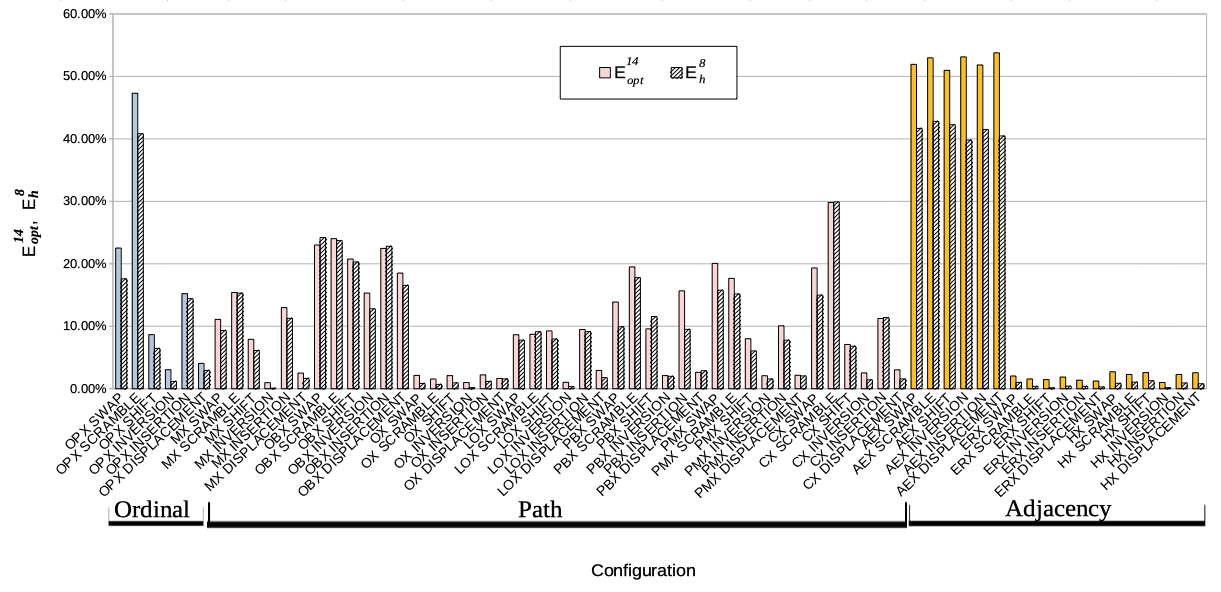
\includegraphics[width=1\textwidth]{10_1_less_100}
	\caption{Results for 22 instances with less than 100 cities for different representation types crossovers combined with 6 mutation operators.}
	\label{fig:10_1_less_100}
\end{sidewaysfigure}	

\begin{sidewaysfigure}[htp] \centering
	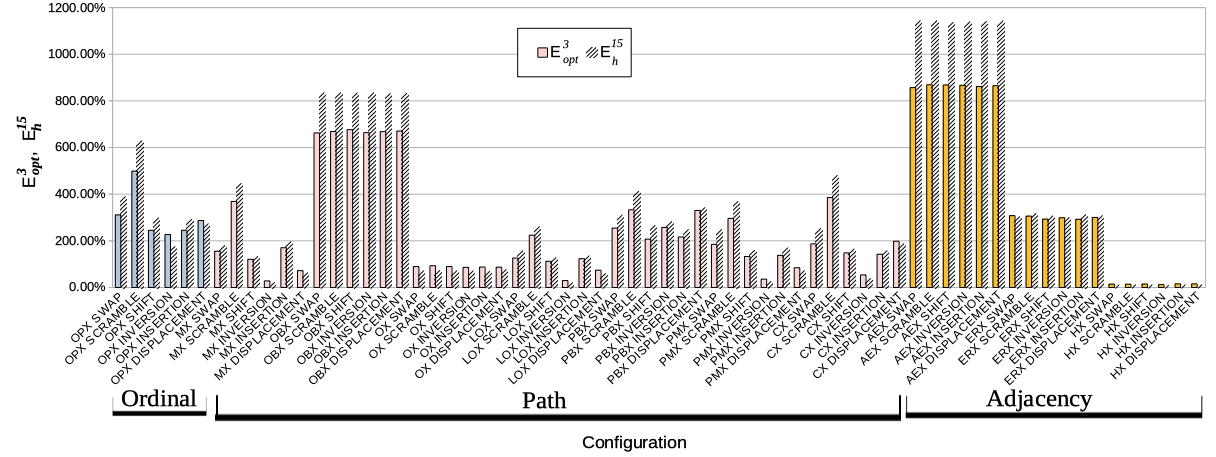
\includegraphics[width=1\textwidth]{10_1_200_to_500}
	\caption{Results for 18 instances with 200 to 500 cities for different representation types crossovers combined with 6 mutation operators.}
	\label{fig:10_1_200_to_500}
\end{sidewaysfigure}

As mentioned before, \citeauthor{potvin1996genetic} \cite{potvin1996genetic} has claimed that the ordinal representation cannot perform well enough to compete with other representation types. However, in our experiments, this representation type has definitely not performed worst. On our dataset which in this experiment included 40 instances, the OPX has outperformed the OBX which has shown the poorest results among the path representation crossovers and the AEX which has shown the poorest results in the group of the adjacency representation crossovers.  However, it could not compete with the crossover operators which have shown the best results, namely the MX, the LOX, the OX, and the HX. Therefore, one can not exclude that the ordinal representation can perform well if, for instance, some specific crossover and mutation operators are developed for it. The ordinal representation  always produces valid offsprings. It therefore does not need additional steps to ensure the validity for the TSP as the path and ordinal representation types do (see Section \ref{subsec:ordinal}). This fact makes this representation type more generally applicable for other combinatorial optimization problems. Therefore, perhaps, the ordinal representation is worth being developed further.\par 

If we take a look at the experiments conducted by \citeauthor{starkweather1991comparison} \cite{starkweather1991comparison}, we can see that in addition to 5 crossover operators of the path representation types (OX, OBX, PBX, PMX, and CX), they launched the ERX as well. This operator has shown much better results in their experiments having achieved the optimum in all 30 trials. Please note that these studies used a single small instance with 30 cities. If we take a look at our experiments for the instances with less that 100 cities (see Figure \ref{fig:10_1_less_100}), we can confirm that the ERX performed better than or comparable to the path representation crossovers.\par 

However, we cannot confirm the claim made by \citeauthor{potvin1996genetic} \cite{potvin1996genetic} that "the edge-preserving operators are superior to the other types of crossover operators". His claim is based on the studies made by \citeauthor{starkweather1991comparison} \cite{starkweather1991comparison} who considered only ERX using only one small instance with 30 cities and on the studies made by \citeauthor{liepins1990genetic} \cite{liepins1990genetic} which used only two types of crossover operators. In our experiment, the AEX performed much worse than all other operators of all groups despite the fact that it is an edge-preserving operator. The ERX has shown a poor performance for instances with 200 to 500 cities as well. Only the HX has performed very good among the edge preserving operators.\par 

\begin{table}[htp] \centering
	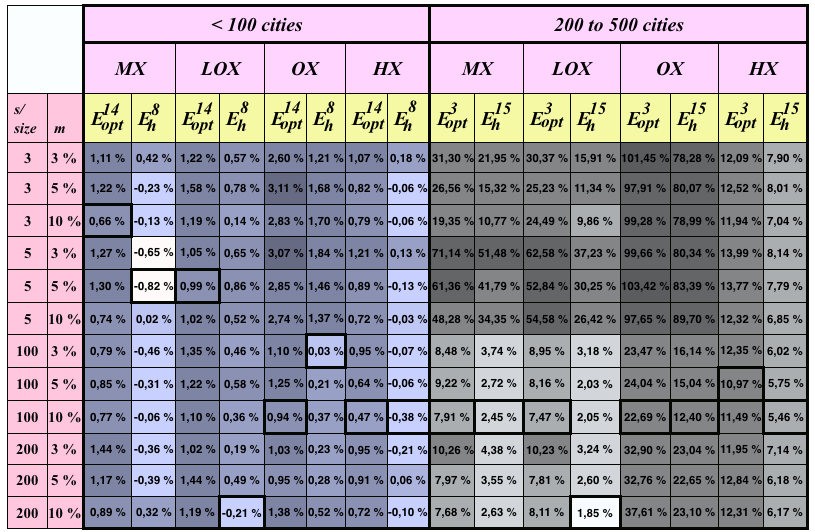
\includegraphics[width=1\textwidth]{tab_10_2_parameter_tuning_without_h}
	\caption{Results for 12 configurations for the MX, LOX, OX, and HX for the random initialization of population, all combined with the inversion mutation.}
	\label{Tab:tab_10_2_parameter_tuning_without_h}
\end{table}	

Now we are going to tune the hyperparameters for the operators which have performed best in the previous experiments, namely the HX, the LOX, the OX, and the MX all combined with the inversion mutation (see Chapter \ref{exp_crossovers}). At first, we have conducted the experiments without using heuristics to initialize the population. It is interesting that the configuration of hyperparameters where the population size was fixed at 100 chromosomes with the mutation rate $10\%$ has performed best for most operators (see Table \ref{Tab:tab_10_2_parameter_tuning_without_h}). However, there are still many different configurations which perform best for a specific operator and  a specific group of instances. Therefore, we conclude that the best configuration of hyperparameters seems to be very sensitive to the size of a TSP instance and the operators used.\par 

\begin{table}[htp] \centering
	\begin{subtable}[t]{0.45\textwidth}
		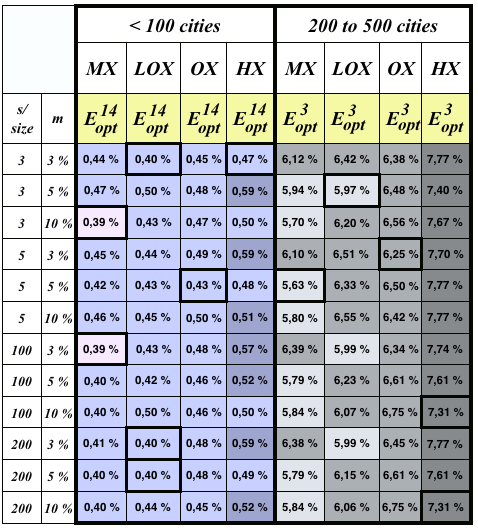
\includegraphics[width=\textwidth]{tab_10_2_parameter_tuning_with_h_opt}
		\caption{Relative error with respect to the optimal value averaged over 14 instances.}
		\label{Tab:tab_10_2_parameter_tuning_with_h_opt}
	\end{subtable}
	\hfill
	\begin{subtable}[t]{0.5\textwidth}
		\centering
		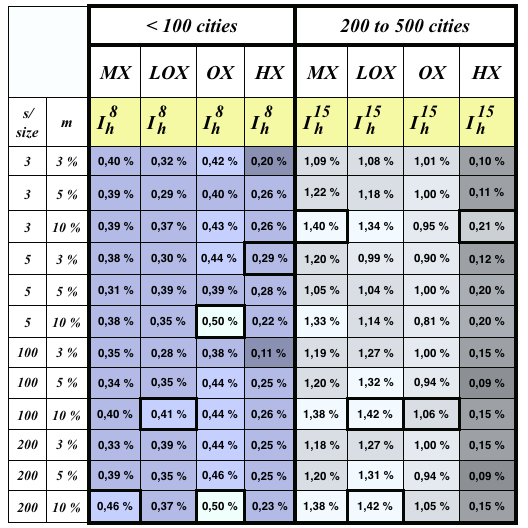
\includegraphics[width=\textwidth]{tab_10_2_parameter_tuning_with_h_vs_h}
		\caption{Relative improvement with respect to the best results of heuristics (with ten minutes limit) averaged over 8 instances.}
		\label{Tab:tab_10_2_parameter_tuning_with_h_vs_h}
	\end{subtable}	
	\caption{Results for 12 configurations for the MX, LOX, OX, and HX for the initialization of population with heuristics, all combined with the inversion mutation.}
	\label{Tab:tab_10_2_parameter_tuning_with_h}
\end{table}


Now let us take a look at the results, where the construction heuristics were used to initialize the population (see Table \ref{Tab:tab_10_2_parameter_tuning_with_h}). Please note that we use the results of heuristics as a benchmark for the instances with no known optimal value. In case of initialization with heuristics, our genetic algorithm can, of course, only outperform the results made by heuristics. Therefore, we will speak about the improvement of the genetic algorithm with respect to the heuristics in this case which we want to maximize (see Figure \ref{Tab:tab_10_2_parameter_tuning_with_h_vs_h}). Here, we can see even higher differentiation concerning the best configuration. This supports our point about the sensibility of the hyperparameters to the size of a TSP instance and the used operators. \par 

Moreover, we can see that the best configuration of parameters for the same operators differs if different types of initializing the population are used (see Tables \ref{Tab:tab_10_2_parameter_tuning_without_h} and \ref{Tab:tab_10_2_parameter_tuning_with_h}). This illustrates that the hyperparameters are sensible not only to the number of cities and the type of operators but to the way how the population is initialized as well.\par 

\begin{table}[htp] \centering
	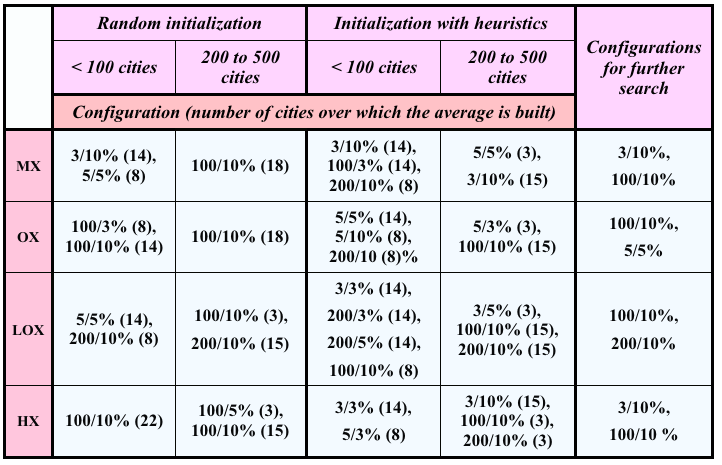
\includegraphics[width=0.7\textwidth]{tab_10_2_best_configs}
	\caption{Best configurations for the MX, LOX, OX, and HX which are all combined with the inversion mutation.}
	\label{Tab:tab_10_2_best_configs}
\end{table}	

\begin{table}[htp] \centering
	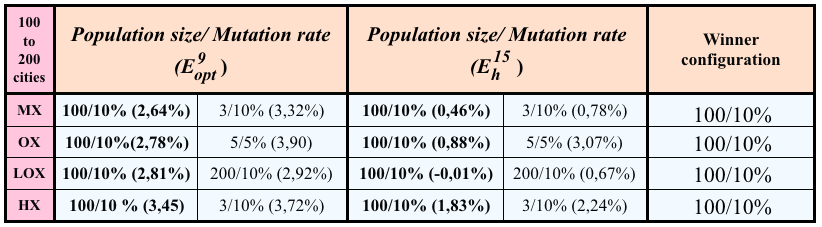
\includegraphics[width=0.7\textwidth]{tab_10_2_winner_configs_random}
	\caption{Winner configurations for the MX, LOX, OX, and HX for random initialization which are all combined with the inversion mutation.}
	\label{Tab:tab_10_2_winner_configs_random}
\end{table}	 

\begin{table}[htp] \centering
	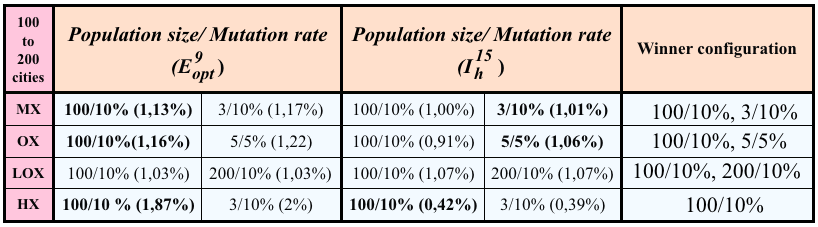
\includegraphics[width=0.7\textwidth]{tab_10_2_winner_configs_h}
	\caption{Winner configurations for the MX, LOX, OX, and HX for initialization with heuristics which are all combined with the inversion mutation.}
	\label{Tab:tab_10_2_winner_configs_h}
\end{table}	 

The best configurations for each crossover operator are given in Table \ref{Tab:tab_10_2_best_configs}. Among them, for each crossover operator, we choose the two combinations which have shown the best results for more instances. If two configurations were the best for the same number of instances, we randomly take one of them. All these chosen configurations were tested on another group of instances which have 100 to 200 cities. The results are given in Tables \ref{Tab:tab_10_2_winner_configs_random} and \ref{Tab:tab_10_2_winner_configs_h}. As one can see, the configuration with the fixed population size at 100 and the mutation rate 10 has performed best for all four operators.\par 

Now we launch the experiments on the remaining two groups of instances, namely the one with 500 to 1500 cities and the one with 1500 to 10000 cities using the selected configurations, namely population size fixed at 100 and the mutation rate of $10\%$ for all four crossover operators. We will get thus the results for the whole dataset. \par 

At first we conducted the experiments without using heuristics to initialize the population. We have to use two benchmarks in our experiments because some instances do not have a known optimal value. As we have five groups of instances, we therefore get 10 charts with the results (see \ref{10_3_final_results_random_init}). For each operator, we calculate the number of charts where it has shown the best results. Overall, the HX has outperformed in 5 subgroups of instances which we can see in the 5 corresponding charts, the LOX is best in 4, the MX has outperformed in 1 case, and the OX was better in none og the subgroups. Of course, some subgroups have very small number of instances, as for instance, there is only one instance with a known optimal value in the group of instances with 1500 to 10000 cities. So the result of $E^{1}_{opt}$ here can be considered as outlier. Therefore, let us calculate instead the number of instances for which the corresponding operator has shown the best averaged results HX: 14 + 1 + 8 + 20 + 14 = 57, LOX: 3 + 3 + 15 + 15 = 36, MX: 9 ,and OX: 0. \par 

Thus, the HX has shown the best results on average independent from the benchmark we used. This is not surprising because the population here includes only random permutations of cities which are more likely to be bad tours. The HX chooses iteratively the shortest edge from the parents which is a very relevant piece of information for the TSP and as a result can significantly improve the initial bad tours. Moreover, the fact that the HX tends to repeat parents for small instances does not seem to impair its performance.\par 

For the instances with number of cities smaller than 200, we can observe negative values of $E_{h}$ which corresponds to an improvement over the heuristics. The genetic algorithm, where the population was initialized only with random permutations, could thus outperform the heuristics despite the relatively short time given, namely ten minutes. Of course, we can see the drastic decrease in performance with the increase in dimension. However, it is important to mention that a stop criterion of ten minutes resulted in much greater number of iterations for the smaller instances than for the larger ones. This means that the genetic algorithm does not necessarily perform much worse on larger instances than on the smaller ones if it gets sufficient time to make the same number of iterations.  \par

It is also important to mention  that the results were averaged over the instances across the corresponding group, and the genetic algorithm was able to find the optimal value for some instances which one cannot see in these charts. \par  

\begin{sidewaysfigure}[htp] \centering
	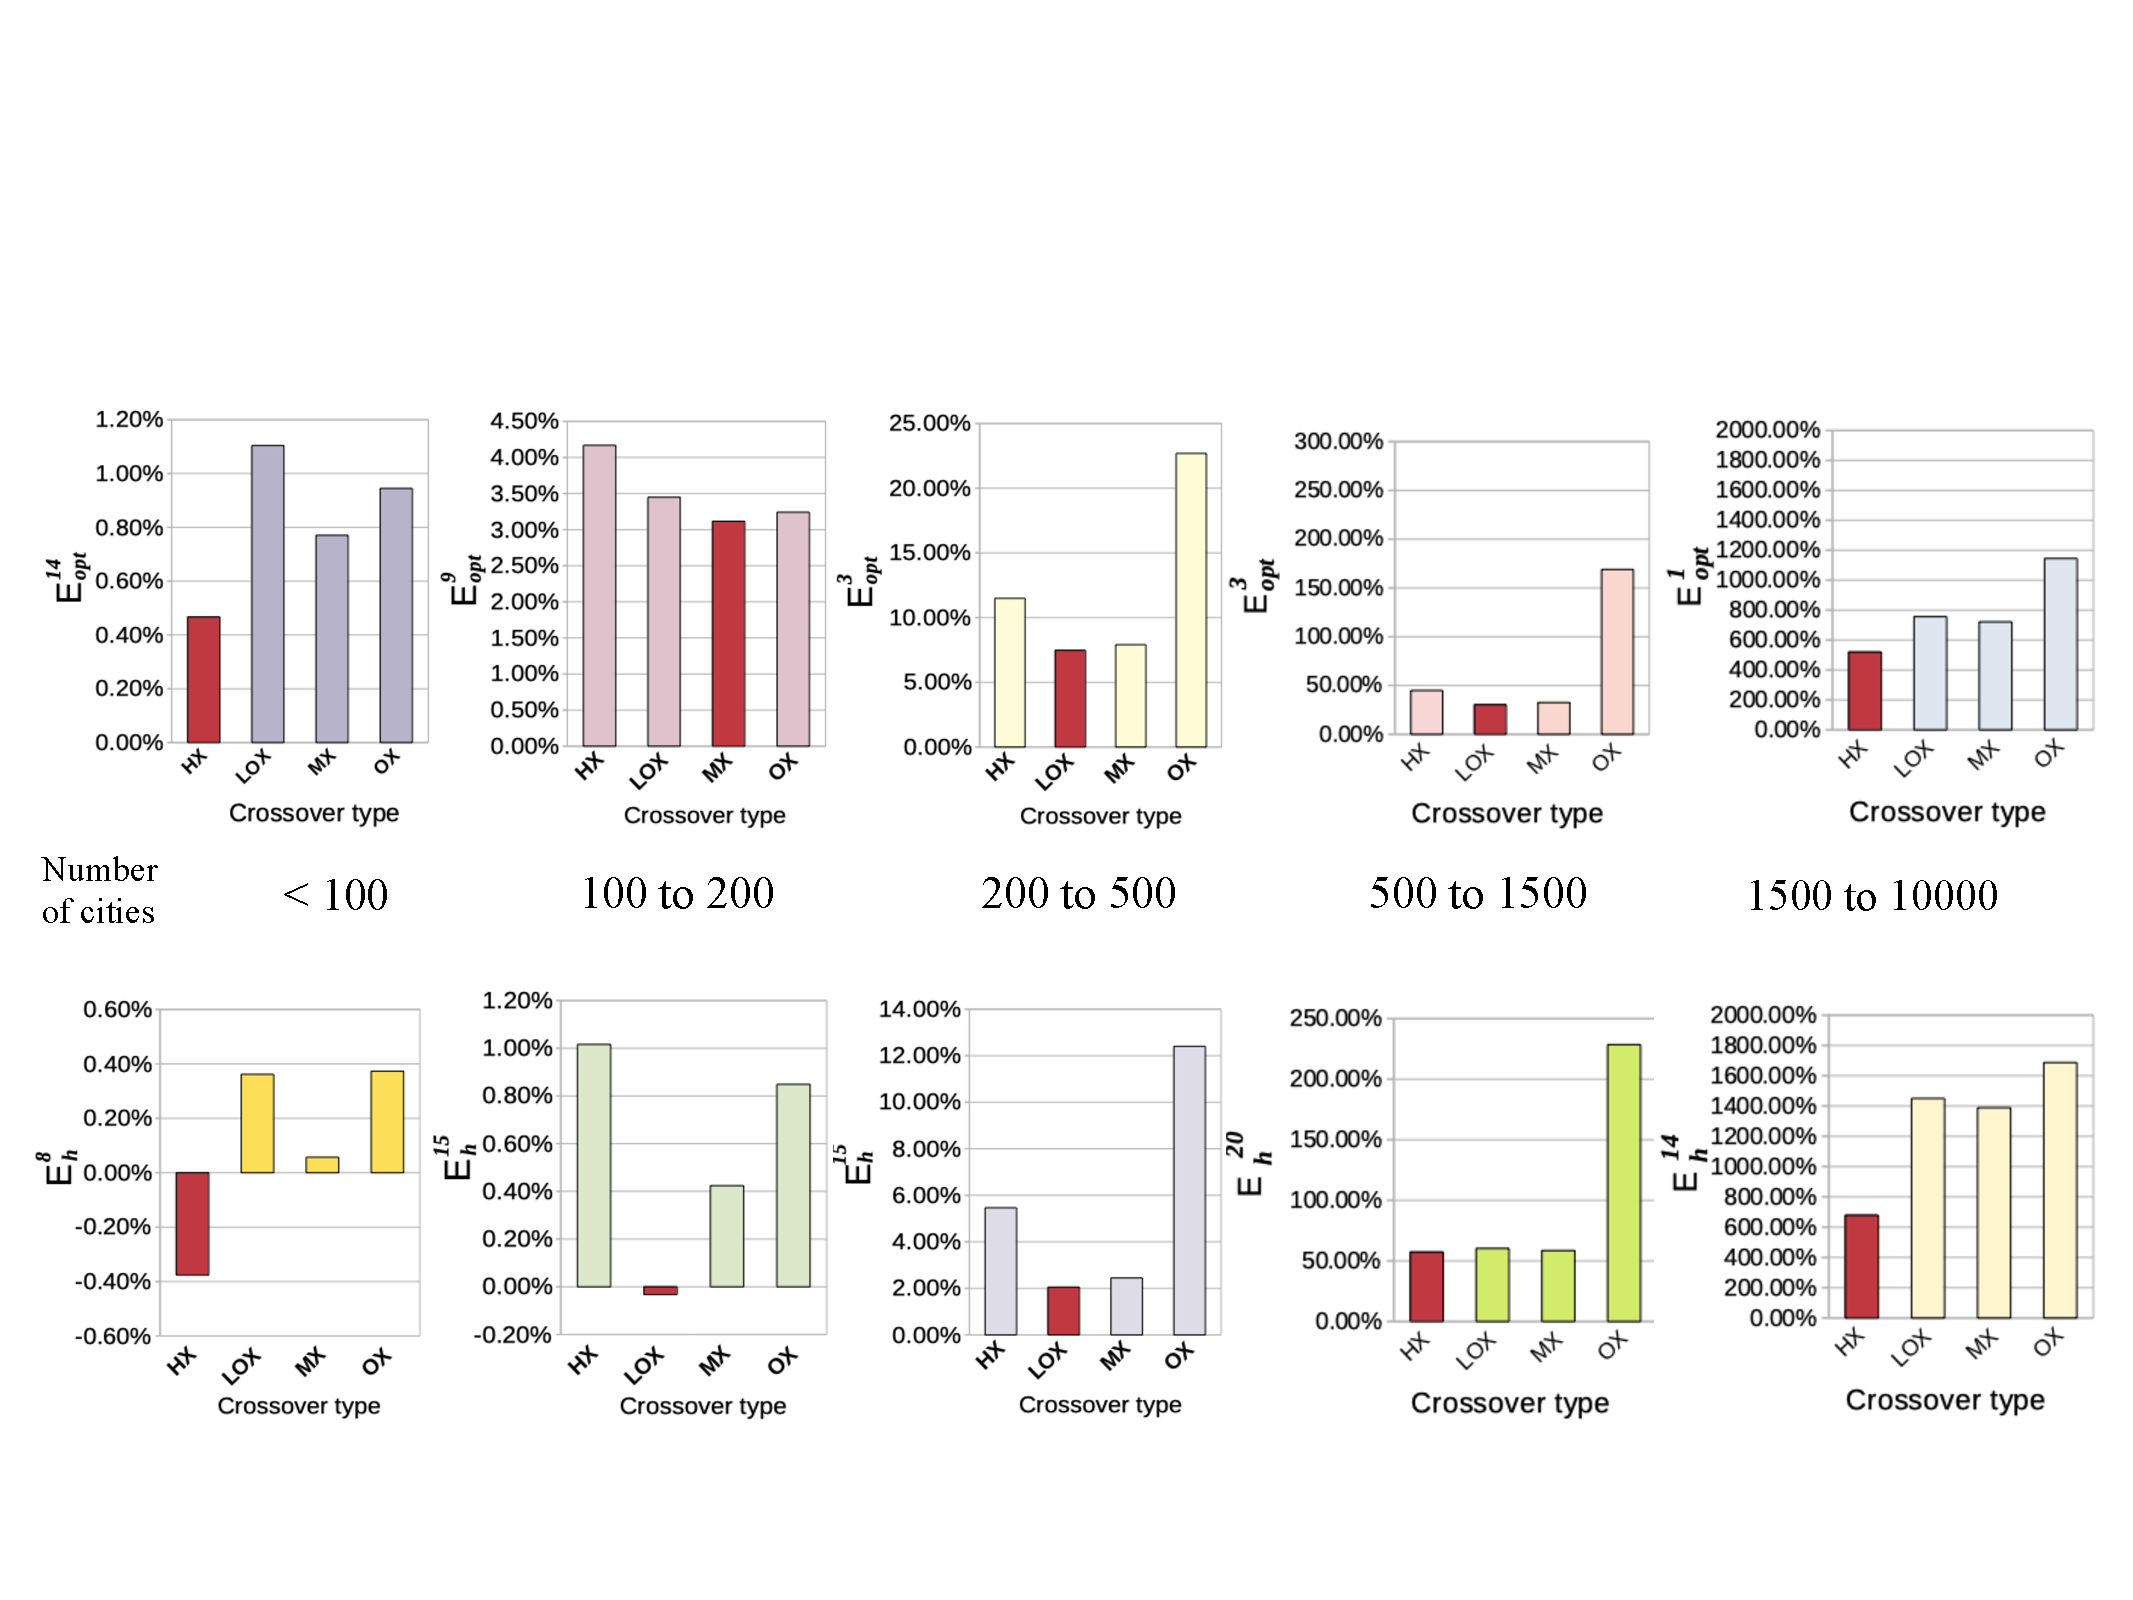
\includegraphics[width=1\textwidth]{10_3_final_results_random_init.pdf}
	\caption{Final results for the MX, LOX, OX, and HX which are all combined with the inversion mutation with the random initialization of population.}
	\label{10_3_final_results_random_init}
\end{sidewaysfigure}

\vspace{2cm}
	
\begin{sidewaysfigure}[htp] \centering
	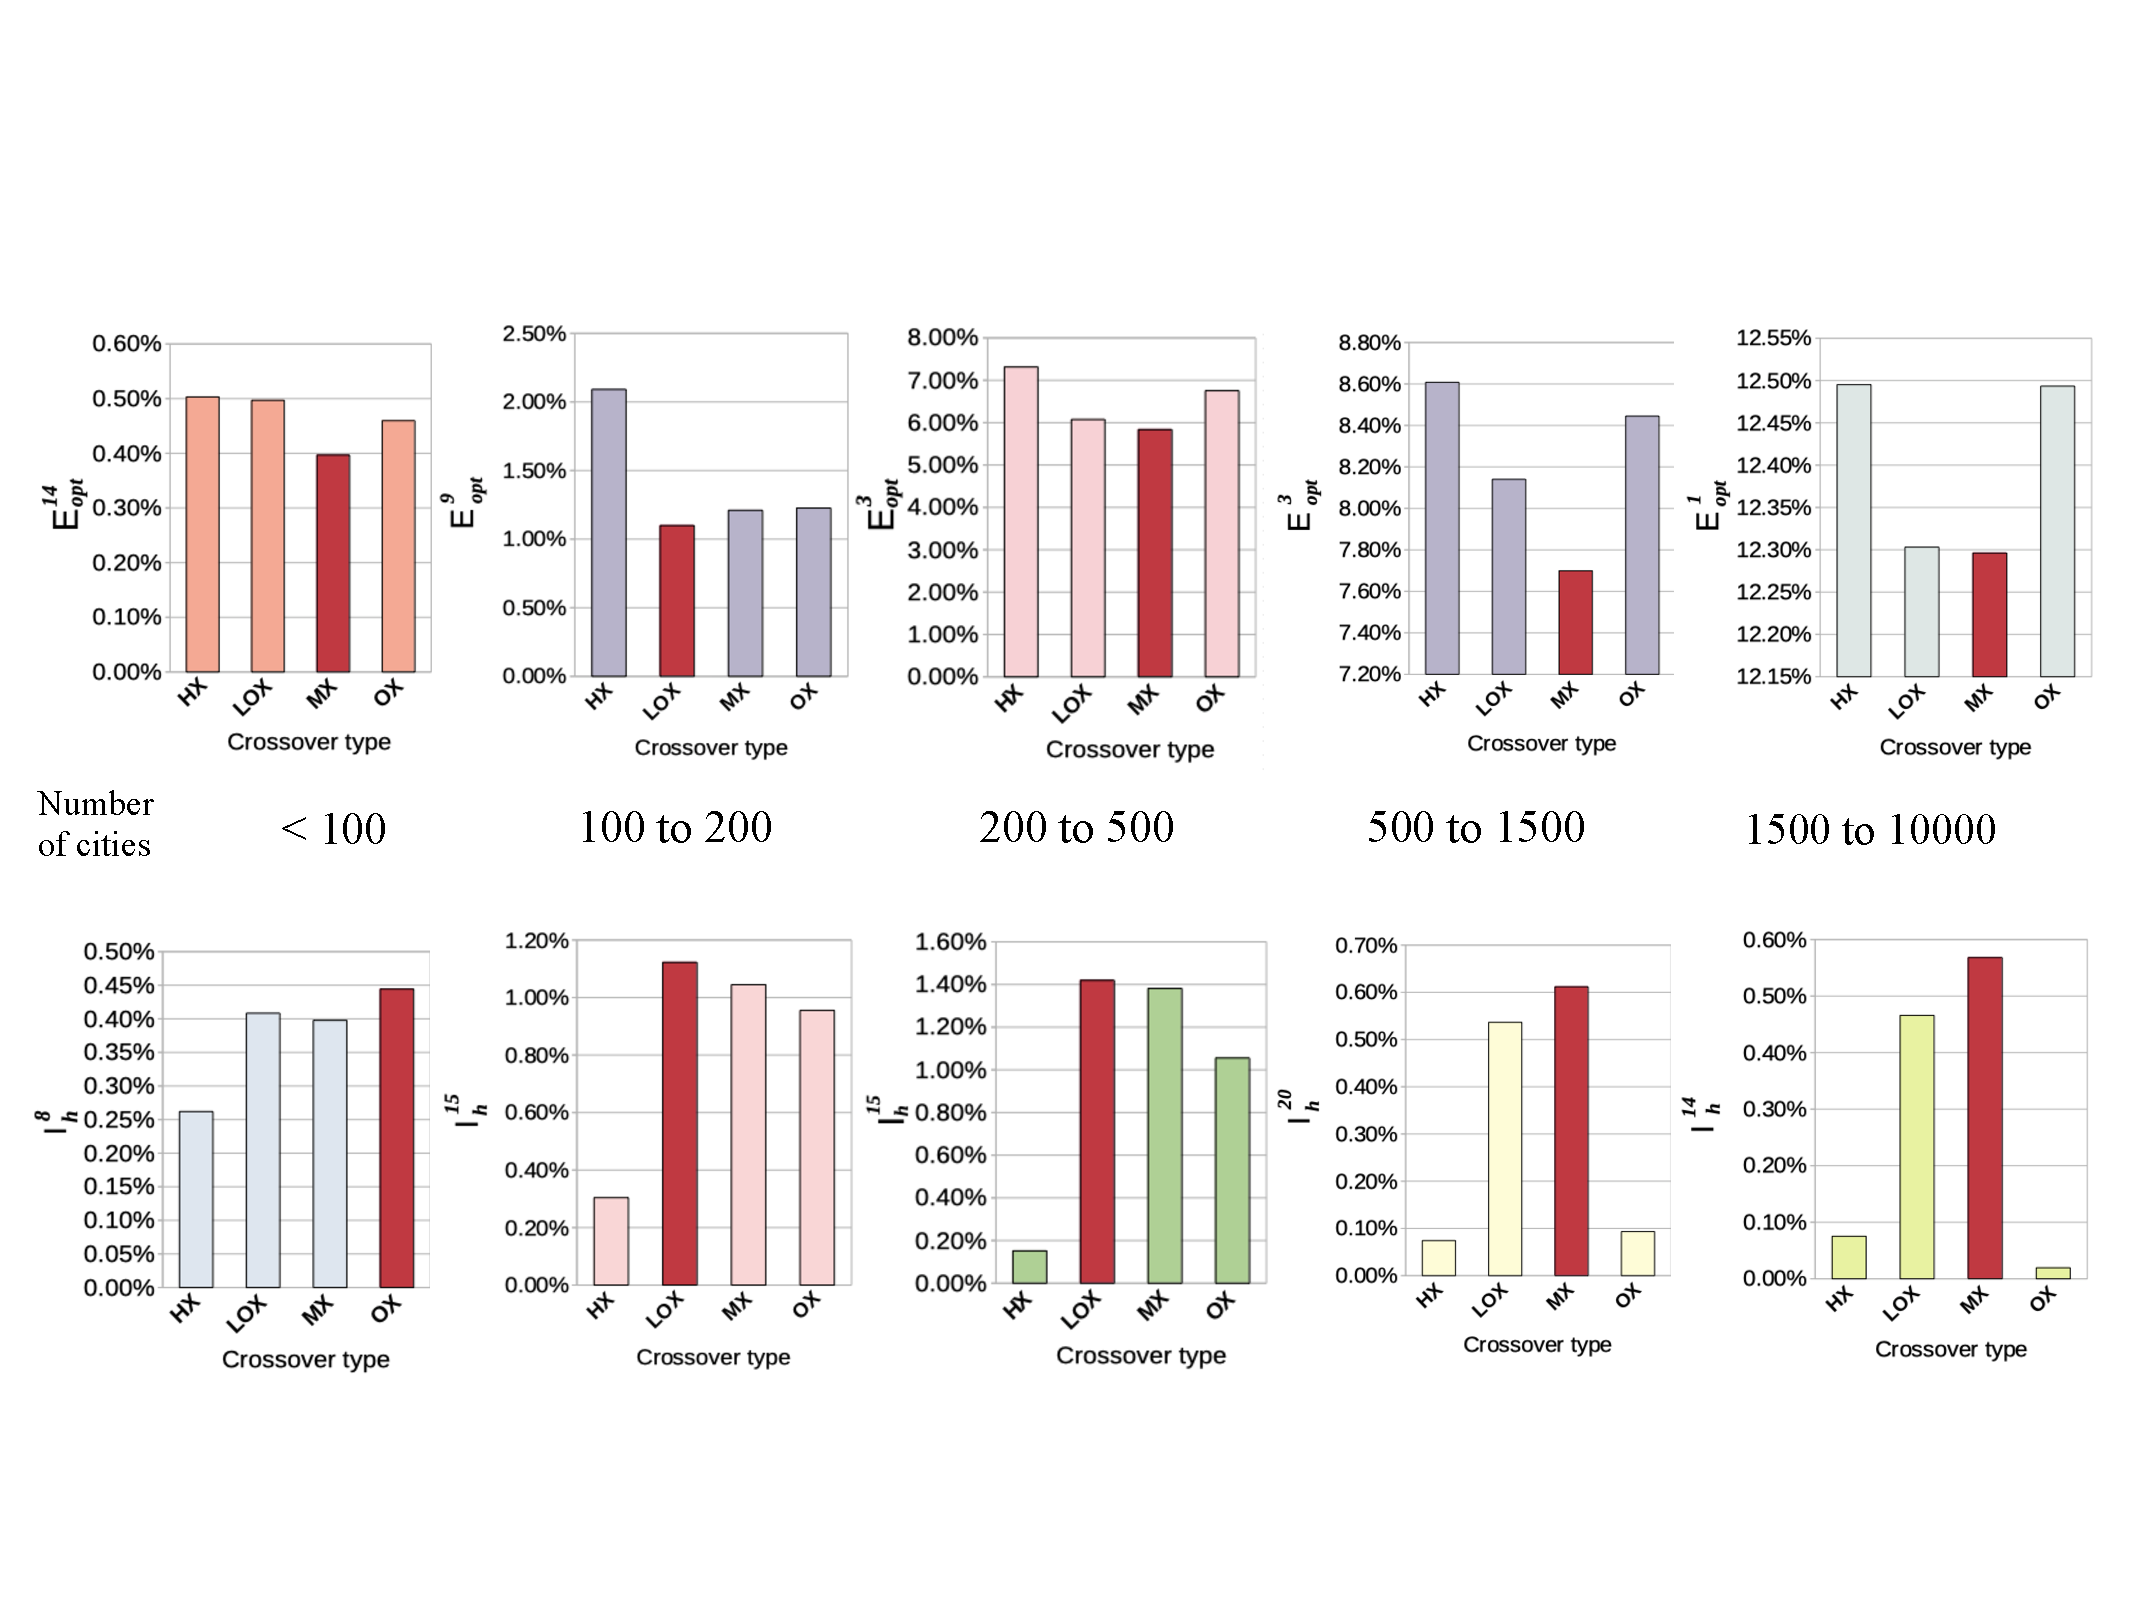
\includegraphics[width=1\textwidth]{10_3_final_results_heuristics_init.pdf}
	\caption{Final results for the MX, LOX, OX, and HX which are all combined with the inversion mutation where the population was initialized using heuristics.}
	\label{10_3_final_results_heuristics_init}
\end{sidewaysfigure}

In the next experiments, we used heuristics to initialize the population (see Figure \ref{10_3_final_results_heuristics_init}). Here, we can notice the decrease in performance with the increase of the number of cities as well. It can be also explained by the fact that for the larger instances, the genetic algorithm could not make sufficient number of iterations in comparison to the smaller instances.\par 

Since the population has been initialized with the results of the construction heuristics, the genetic algorithm can not physically perform worse than the heuristics. Therefore, the relative improvement over the heuristics is considered in this case, and it is maximized.\par 

The MX has outperformed in 7 subgroups of instances which we can see in the 6 corresponding charts, the LOX in 3, the OX in 1, and the HX was best in none of the subgroups.  If we calculate the number of instances for which the corresponding operator was on average the best, we have MX: 14 + 3 + 3 + 1 + 20 + 14 = 55, LOX: 9 + 15 + 15 = 39, OX: 8, and HX: 0.\par 

 It is interesting that the HX here has shown worse results while the MX is the definite winner. As it was described in Section \ref{subsec:path_crossovers}, the MX makes the simplest changes in comparison to the other crossovers and results therefore in more iterations per time unit. Its great performance here can be explained by the fact that the heuristics used in the population have already come to very good results: The domain information is already used, and the HX cannot offer much in this case but requires more computations and thus more time. The MX, however, makes rather random changes but it makes them much faster. As a result, it slightly improves the initial results of the heuristics.\par 	

It is interesting to mention that in these experiments, where the population size was fixed at 100 chromosomes, and the mutation rate was $10\%$, the OX has performed constantly worse than the LOX. This is exactly the opposite tendency in comparison with the one we reported in Section \ref{subsec:experiments_path}, where we multiplied the number of cities by the factor 3 to get the population size, and where the mutation rate was $3\%$. Therefore, we can conclude that the choice of parameters plays an important role in performance of genetic algorithms.\par 

Considering the two approaches which we used to initialize the population, we can definitely claim that using heuristics in the population improves the performance of the genetic algorithm. For all groups of instances, the results are better when the heuristics are used, and the difference in performance becomes especially visible with the increase of dimension. So, if we work with rather small instances which have less than 100 cities, for instance, the best value  with random initialization is $E^{14}_{opt} = 0.47 \%$, with the HX used. The best value achieved in this case with using heuristics is $E^{14}_{opt} = 0.40\%$ with the MX. So, the difference here probably does not justify implementing and using the heuristics. The results obtained with the random initialization of the population can be considered as sufficient. But if we work with large instances, the difference is drastic. For instance, if we take a look at the group of instances with 500 to 1500 cities, the best result is $E^{3}_{opt} = 30.36\%$ achieved by the LOX for random initialization while the best relative error  for the initialization with heuristics is $E^{3}_{opt} = 7.70\%$ achieved with the MX. Therefore, it definitely makes sense to include the results of heuristics into the initial population if one works with large instances or if even a slightly improvement in performance for smaller instances is important.\par 
